
%%%%%%%%%%%%%%%%%%%%%%%%%%%%%%%%%%%%%%%%%%%%%%%%%%%%%%%%%%%%%%%%%%%%%%%%%%%%%%%%%%%%%%%%%%%%%%%%%%%%%%%%%%%
%%%%%%%%%%%%%%%%%%%%%%%%%%%%%%%%%%%%%%%%%%%%%%%%%%%%%%%%%%%%%%%%%%%%%%%%%%%%%%%%%%%%%%%%%%%%%%%%%%%%%%%%%%%
%%
%% This is the template for writing Thesis in LaTeX for the Graduate Students of King Fahd University of
%% Petroleum & Minerals, Dhahran, K.S.A.
%%
%% All the Comments are written with the line starting with '%%'. They should not be removed.
%%
%% Please make sure to have the class file named: 'kfupm_thesis.cls'. PLEASE DO NOT ALTER IT!
%%
%% Carefully read the comments in the following documnent and add/edit only where mentioned.
%%
%% In order to enable a line remove the preceeding '%' sign and to disable a line insert '%' at the start.
%%
%% Please make sure that you have the compatible versions of MikTex installed prioir to using this
%% template.
%%
%% Go through the Thesis Writing manual and the Latex guidelines document available at the DGS website.
%%
%%%%%%%%%%%%%%%%%%%%%%%%%%%%%%%%%%%%%%%%%%%%%%%%%%%%%%%%%%%%%%%%%%%%%%%%%%%%%%%%%%%%%%%%%%%%%%%%%%%%%%%%%%%
%%%%%%%%%%%%%%%%%%%%%%%%%%%%%%%%%%%%%%%%%%%%%%%%%%%%%%%%%%%%%%%%%%%%%%%%%%%%%%%%%%%%%%%%%%%%%%%%%%%%%%%%%%%
%% Always ensure that only one \documentclass{} line is enabled at one time

%% For MS Thesis enable the next line

\documentclass[ms,twoside, 12pt]{kfupm_thesis}

%For green card title page enable the following line
%\documentclass[printready,ms,twoside, 12pt]{kfupm_thesis}

%% For PhD Thesis enable the next line

%\documentclass[phd,twoside, 12pt]{class_bst/kfupm_thesis}
%\documentclass[phd,twoside, 12pt]{kfupm_thesis}
%For green card title page enable the following line
%\documentclass[printready,phd,twoside, 12pt]{kfupm_thesis}

%%%%%%%%%%%%%%%%%%%%%%%%%%%%%%%%%%%%%%%%%%%%%%%%%%%%%%%%%%%%%%%%%%%%%%%%%%%%%%%%%%%%%%%%%%%%%%%%%%%%%%%%%%%

% The following file defines margins and text width

\textwidth=5.75in
\oddsidemargin=0.505in


%%%%%%%%%%%%%%%%%%%%%%%%%%%%%%%%%%%%%%%%%%%%%%%%%%%%%%%%%%%%%%%%%%%%%%%%%%%%%%%%%%%%%%%%%%%%%%%%%%%%%%%%%%%
% The following file defines the inclusion of packages and some other required commands

%%%%%%%%%%%%%%%%%%%%%%%%%%%%%%%%%%%%%%%%%%%%%%%%%%%%%%%%%%%%%%%%%%%%%%%%%%%%%%%%%%%%%%%%%%%%%%%%%%%%%%%%%%%

%% The following is the list of most commonly used packages. If more / other packages are needed they are
%% to be added immediately after the following list.
\usepackage{graphicx}
\usepackage{latexsym}
\usepackage{amsmath,epsfig}
%\usepackage{epstopdf}

\usepackage{graphicx}
\usepackage{epsfig}
\usepackage{graphicx}
\usepackage{latexsym}
\usepackage{amsmath}
\usepackage{amssymb}
\usepackage{mhsetup}
\usepackage{mathtools}
\usepackage{mathrsfs}
\usepackage{float}
\usepackage{xfrac}
\usepackage{epsfig}

%The polyglossia package allows for using Arabic and English together in one document.
%IMPORTANT: polyglossia is only compatible with XeLaTeX
\usepackage{polyglossia}%
\setmainlanguage{english}%
%This handles a bug due to polyglossia which corrupts the \maketitle command in hyperref
\let\keptmaketitle\maketitle%
%This allows navigation using links
\usepackage{hyperref}
\hypersetup{
	colorlinks,
	citecolor=blue,
	filecolor=blue,
	linkcolor=black,
	urlcolor=blue,
	%hidelinks=false %use this to change color of hyperlinks
}
%This package is used to get the correct formatting of the list of abbreviations and list of symbols using glossaries
\usepackage{enumitem}
%--------------------------------------------------
% Needed to insert empty page between title and committe page in double sided document
\newcommand{\clearemptydoublepage}{%
  \clearpage
  {\pagestyle{empty}\cleardoublepage}%
}
%--------------------------------------------------

%% The following is required for References

\addto{\captionsenglish}{%
  \renewcommand{\bibname}{REFERENCES}
  }	

%% Thefollowing are the most common figure file extensions

\DeclareGraphicsExtensions{.pdf,.png,.jpg, .eps}

%add
\usepackage{comment}
\graphicspath{{./figs/}}
\usepackage{import}
\makeatletter
\def\input@path{{./bst/}}
\makeatother
\usepackage{lipsum}

%%%%%%%%%%%%%%%%%%%%%%%%%%%%%%%%%%%%%%%%%%%%%%%%%%%%%%%%%%%%%%%%%%%%%%%%%%%%%%%%%%%%%%%%%%%%%%%%%%%%%%%%%%%
% The following file defines the settings for including List of Abbreviations

%%%%%%%%%%%%%%%%%%%%%%%%%%%%%%%%%%%%%%%%%%%%%%%%%%%%%%%%%%%%%%%%%%%%%%%%%%%%%%%%%%%%%%%%%%%%%%%%%%%%%%%%%%%

%% The following is used for the insertion of the List of Abbreviations. If this is to be used then enable
%% the following 3 lines.

%\usepackage{nomencl}
%
%\makenomenclature
%
%\renewcommand{\nomname}{LIST OF ABBREVIATIONS}

%%%%%%%%%%%%%%%%%%%%%%%%%%%%%%%%%%%%%%%%%%%%%%%%%%%%%%%%%%%%%%%%%%%%%%%%%%%%%%%%%%%%%%%%%%%%%%%%%%%%%%%%%%%
%glossaries package for list of symbols and list of abbreviations
\usepackage[xindy,toc,acronym,nonumberlist,nopostdot]{glossaries}
\renewcommand*{\glsclearpage}{}% to remove empty pages before the list of abbreviations and list of symbols

%%%%%%%%%%%%%%%%%%%%%%%%%%%%%%%%%%%%%%%%%%%%%%%%%%%%%%%%%%%%%%%%%%%%%%%%%%%%%%%%%%%%%%%%%%%%%%%%%%%%%%%%%%%
% The following file defines the list of abbreviations


%
%\addcontentsline{toc}{chapter}{\, \, \, LIST OF ABBREVIATIONS}{\pageref{LOA}}
%
%\label{LOA}
%
%%% The following should contain the list of all abbreviations to be used in the Thesis write-up. Enter the
%%% the abbreviations and their full form as shown below for example.
%
%\nomenclature{LED}{Light Emitting Diode}
%\nomenclature{MOS}{Metal Oxide Semiconductor}
%\nomenclature{PC}{Personal Computer}
%
%\printnomenclature [2.5 cm]
%to use the glossaries package, the symbols and acronyms have to be defined first
%SYMBOLS: Symbols can be defined using the following code
\newcommand{\sym}[4]{%This command can be used to define a symbol as explain below
	\newglossaryentry{#1}{%
		name={#2},
		description={#3},
		symbol={#2},
		sort={#4}
	}%
}%
%The format for defining a symbol is as follows
%\sym{label}{symbol}{description}{alphabetical sorting name}
%label: This will be used later on in the main body to use the symbol
%symbol: The actual symbol to be used
%description: The description of the symbol
%alphabetical sorting name: This name will be used to sort the symbol in alphabetical order if desired
%example symbol definition
\sym{mysymbol}{\ensuremath{\Gamma}}{This is a symbol}{gamma}
\sym{yoursymbol}{\ensuremath{\Theta}}{This is a symbol}{tetha}

%An acronym or abbreviation can be defined as follows
%\newacronym{label}{short}{long}
%label: this will be used to call the acronym in the main body
%short: the acronym
%long: the full form of the acronym
%example acronym
\newacronym{phd}{Ph.D.}{Doctor of Philosophy}
\newacronym{uav}{UAV}{Unmanned Aerial Vehicle}
\newacronym{vrp}{VRP}{Vehicle Routing Problem}

\makeglossaries
%%%%%%%%%%%%%%%%%%%%%%%%%%%%%%%%%%%%%%%%%%%%%%%%%%%%%%%%%%%%%%%%%%%%%%%%%%%%%%%%%%%%%%%%%%%%%%%%%%%%%%%%%%%
\setotherlanguage{arabic} %
\newfontfamily\arabicfont[Script=Arabic]{Scheherazade} 
%We have to define an Arabic font
\let\maketitle\keptmaketitle %

%---------------------------------------------------
%added to overcome the text strecting from top to bottom when using openright
\raggedbottom%
%--------------------------------------------------------
\begin{document}
%%%%%%%%%%%%%%%%%%%%%%%%%%%%%%%%%%%%%%%%%%%%%%%%%%%%%%%%%%%%%%%%%%%%%%%%%%%%%%%%%%%%%%%%%%%%%%%%%%%%%%%%%%%
% The following file defines the title, author, advisers etc.

%% Please enter the Complete Title of the Thesis / Dissertation

\title{your thesis tittle}

%% Please enter the Complete Name of the Author

\author{your name}

%% Please enter the Complete Name of the Major (NOT Department, unless if they are the same) e.g. \dept{Electrical Engineering}

\dept{INDUSTRIAL AND SYSTEM ENGINEERING}

%% Please enter the Month and Year of Thesis / Dissertation

\date{DECEMBER 2025}

%adding data for arabic abstract
%title in arabic added 
\artitle{عنوان الرسالة}

%name in arabic added
\arname{اسم الطالب}

%department in arabic added 
\ardept{قسم الطلاب}
%% Please enter the Month and Year of Thesis / Dissertation

%date in arabic added 
\ardate{أدخل الشهر والسنة}
\maketitle

%% Please enter the Complete Name of the Advisor

\adviser{Advisor}

%% Please enter the Complete Name of the Co-Advisor if you have a Co-Adviser else comment it out.

%\coadviser{Dr. }

%% Please enter the Complete Name of the Committee Member

\memberone{Member 1}

%% Please enter the Complete Name of the Committee Member

\membertwo{Member 2}

%% Please enter the Complete Name of the Committee Member

\memberthree{Member 3}

%% Please enter the Complete Name of the Committee Member

\memberfour{Member 4}

%% Please enter the Complete Name of the Department Chairman

\chairman{Chaiman}

%% Please enter the Complete Name of the Dean of Graduate Studies

%\deanGS{Dr. Salam A. Zummo}
\deanGS{Dr. Suliman Al-Homidan}

%%%%%%%%%%%%%%%%%%%%%%%%%%%%%%%%%%%%%%%%%%%%%%%%%%%%%%%%%%%%%%%%%%%%%%%%%%%%%%%%%%%%%%%%%%%%%%%%%%%%%%%%%%%
%% Note: The committee page will be made based on the names entered above
%-------------------------------------------------
% Changes by Waqas
\clearemptydoublepage%needed in double sided documents
\MakeCommitteeCertificate%

%The following commands are not needed any more unless a master student wants to make a five member committee without a co advisor then he can use the MakeCertificatefive command
%\MakeCertificateThree %
%\MakeCertificateFive %
%------------------------------------------------------
\thispagestyle{plain}

%%%%%%%%%%%%%%%%%%%%%%%%%%%%%%%%%%%%%%%%%%%%%%%%%%%%%%%%%%%%%%%%%%%%%%%%%%%%%%%%%%%%%%%%%%%%%%%%%%%%%%%%%%%
%%%%%%%%%%%%%%%%%%%%%%%%%%%%%%%%%%%%%%%%%%%%%%%%%%%%%%%%%%%%%%%%%%%%%%%%%%%%%%%%%%%%%%%%%%%%%%%%%%%%%%%%%%%


%%%%%%%%%%%%%%%%%%%%%%%%%%%%%%%%%%%%%%%%%%%%%%%%%%%%%%%%%%%%%%%%%%%%%%%%%%%%%%%%%%%%%%%%%%%%%%%%%%%%%%%%%%%
% The following file defines the copyright


\newpage
\begin{center}
\text{}
\end{center}
\begin{center}
\text{}
\end{center}
\begin{center}
\text{}
\end{center}
\begin{center}
\text{}
\end{center}
\begin{center}
\text{}
\end{center}
\begin{center}
\text{}
\end{center}
\begin{center}
\text{}
\end{center}
\begin{center}
\text{}
\end{center}
\begin{center}
\text{}
\end{center}

\begin{center}
{\large {\copyright Your Name \\
2025
}}
\end{center}

%%%%%%%%%%%%%%%%%%%%%%%%%%%%%%%%%%%%%%%%%%%%%%%%%%%%%%%%%%%%%%%%%%%%%%%%%%%%%%%%%%%%%%%%%%%%%%%%%%%%%%%%%%%
%%%%%%%%%%%%%%%%%%%%%%%%%%%%%%%%%%%%%%%%%%%%%%%%%%%%%%%%%%%%%%%%%%%%%%%%%%%%%%%%%%%%%%%%%%%%%%%%%%%%%%%%%%%


%%%%%%%%%%%%%%%%%%%%%%%%%%%%%%%%%%%%%%%%%%%%%%%%%%%%%%%%%%%%%%%%%%%%%%%%%%%%%%%%%%%%%%%%%%%%%%%%%%%%%%%%%%%
% The following file defines the dedication page


\newpage
\topskip0pt
\vspace*{\fill}
\begin{center}
{\large \emph{Dedication}}
\end{center}
\vspace*{\fill}

%%%%%%%%%%%%%%%%%%%%%%%%%%%%%%%%%%%%%%%%%%%%%%%%%%%%%%%%%%%%%%%%%%%%%%%%%%%%%%%%%%%%%%%%%%%%%%%%%%%%%%%%%%%
%%%%%%%%%%%%%%%%%%%%%%%%%%%%%%%%%%%%%%%%%%%%%%%%%%%%%%%%%%%%%%%%%%%%%%%%%%%%%%%%%%%%%%%%%%%%%%%%%%%%%%%%%%%


%%%%%%%%%%%%%%%%%%%%%%%%%%%%%%%%%%%%%%%%%%%%%%%%%%%%%%%%%%%%%%%%%%%%%%%%%%%%%%%%%%%%%%%%%%%%%%%%%%%%%%%%%%%
% The following file defines the acknowledgments

\newpage%

\Acknowledgements{
\begin{center}
\noindent \emph{It's customary and good manners to say thank you. Keep in mind that one has to use one's own words when writing an acknowledgement. It's customary and good manners to say thank you. Keep in mind that one has to use one's own words when writing an acknowledgement.}

\emph{It's customary and good manners to say thank you. Keep in mind that one has to use one's own words when writing an acknowledgement. It's customary and good manners to say thank you. Keep in mind that one has to use one's own words when writing an acknowledgement.}
\end{center}
}

%%%%%%%%%%%%%%%%%%%%%%%%%%%%%%%%%%%%%%%%%%%%%%%%%%%%%%%%%%%%%%%%%%%%%%%%%%%%%%%%%%%%%%%%%%%%%%%%%%%%%%%%%%%

\begin{preamble}

%Printing list of symbols and abbreviations
%setting the width of the labels the same as 2.5cm as required by DGS template
\setlist[description]{leftmargin=!, labelwidth=2.5cm, font=\normalfont} %
{
\setstretch{1.5}%
%
\newpage
\phantomsection
\printglossary[title=LIST OF SYMBOLS, toctitle=LIST OF SYMBOLS, nogroupskip] %
%
\newpage%
\phantomsection
\printglossary[title=LIST OF ABBREVIATIONS, toctitle=LIST OF ABBREVIATIONS,type=\acronymtype,nogroupskip] %
\setstretch{2}%
}
\setlist[description]{style=standard} %
%
% The following file defines the Thesis abstract
\textwidth=5.75in
\oddsidemargin=0.505in


\end{preamble}

%%%%%%%%%%%%%%%%%%%%%%%%%%%%%%%%%%%%%%%%%%%%%%%%%%%%%%%%%%%%%%%%%%%%%%%%%%%%%%%%%%%%%%%%%%%%%%%%%%%%%%%%%%%
% The following file defines the contents of Chapter One of the Thesis
\newpage
\setstretch{2}
\chapter{introduction}
\label{ch1}
    \section{Overview and Motivation}
    \label{sec1.1}
    This is sec1.1
\lipsum[2-4]


    \section{Problem Statement}
    \label{sec1.2}
    This is sec1.2
    
    \section{Dissertation Organization}
    \label{sec1.3}
    This is sec1.3

%%%%%%%%%%%%%%%%%%%%%%%%%%%%%%%%%%%%%%%%%%%%%%%%%%%%%%%%%%%%%%%%%%%%%%%%%%%%%%%%%%%%%%%%%%%%%%%%%%%%%%%%%%%
% The following file defines the contents of Chapter Two of the Thesis
\newpage
\chapter{title}
\label{ch2}
    \section{Section Title}
    \label{sec2.1}
    \gls{phd} \gls{uav} \lipsum[1-4]

%%%%%%%%%%%%%%%%%%%%%%%%%%%%%%%%%%%%%%%%%%%%%%%%%%%%%%%%%%%%%%%%%%%%%%%%%%%%%%%%%%%%%%%%%%%%%%%%%%%%%%%%%%%
% The following file defines the appendices if needed

\newpage%
\appendix%
\chapter{Proofs} %Appendix A
\chapter{Supplementary Material} %Appendix B

%%%%%%%%%%%%%%%%%%%%%%%%%%%%%%%%%%%%%%%%%%%%%%%%%%%%%%%%%%%%%%%%%%%%%%%%%%%%%%%%%%%%%%%%%%%%%%%%%%%%%%%%%%%
% The following file defines the inclusion of the References used in the Thesis

%%%%%%%%%%%%%%%%%%%%%%%%%%%%%%%%%%%%%%%%%%%%%%%%%%%%%%%%%%%%%%%%%%%%%%%%%%%%%%%%%%%%%%%%%%%%%%%%%%%%%%%%%%%
%%%%%%%%%%%%%%%%%%%%%%%%%%%%%%%%%%%%%%%%%%%%%%%%%%%%%%%%%%%%%%%%%%%%%%%%%%%%%%%%%%%%%%%%%%%%%%%%%%%%%%%%%%%

%\newpage

%%%%%%%%%%%%%%%%%%%%%%%%%%%%%%%%%%%%%%%%%%%%%%%%%%%%%%%%%%%%%%%%%%%%%%%%%%%%%%%%%%%%%%%%%%%%%%%%%%%%%%%%%%%

\newpage

\phantomsection % This ensures correct numbering in the table of contents
\addcontentsline{toc}{chapter}{REFERENCES}%Add Acknowledgements to the table of contents as a clickable link with hyperref package
\label{references}
%\addtocontents{toc}{\contentsline{chapter}{\numberline{}REFERENCES}{\pageref{references}}}\label{references}
\bibliographystyle{bst/IEEEtran}
\bibliography{3_last/3_library}

%%%%%%%%%%%%%%%%%%%%%%%%%%%%%%%%%%%%%%%%%%%%%%%%%%%%%%%%%%%%%%%%%%%%%%%%%%%%%%%%%%%%%%%%%%%%%%%%%%%%%%%%%%%
%%%%%%%%%%%%%%%%%%%%%%%%%%%%%%%%%%%%%%%%%%%%%%%%%%%%%%%%%%%%%%%%%%%%%%%%%%%%%%%%%%%%%%%%%%%%%%%%%%%%%%%%%%%


%%%%%%%%%%%%%%%%%%%%%%%%%%%%%%%%%%%%%%%%%%%%%%%%%%%%%%%%%%%%%%%%%%%%%%%%%%%%%%%%%%%%%%%%%%%%%%%%%%%%%%%%%%%
% The following file defines the CV of the student

\newpage
\phantomsection % This ensures correct numbering in the table of contents
\addcontentsline{toc}{chapter}{VITAE}%Add Acknowledgements to the table of contents as a clickable link with hyperref package
\label{vitae}
%\addtocontents{toc}{\contentsline{chapter}{\numberline{}VITAE}{\pageref{vitae}}}\label{vitae}
%\begin{center}
%\textbf{\centerline{\huge Vitae}}\end{center}
%\bigskip\bigskip\bigskip

\chapter*{\centering VITAE}
%\vspace*{-1em}

%% Please enter the personal details of the author in the following in place of xxxxx

\begin{itemize}
  \item Name\hspace{3.11cm}: Your Name  		
  \item Nationality\hspace{2.12cm}: Indonesian	
  \item Date of Birth\hspace{1.72cm}: $2^{nd}$ of January 2000
  \item Email\hspace{3.08cm}: \emph{\href{mailto:xxx.yyy@gmail.com}{xxx.yyy@gmail.com}}
  \item Permanent Address\hspace{0.62cm}: Indonesia
  %\newline
%%
%% Please enter the education background in the following
%%
  \item Academic Background\hspace{0.1cm}: 1) Bachelor's degree in Industrial Engineering from MIT in 2030. 2) Master's Degree in Industrial Engineering and Management from Harvard, Indonesia, in 2050.
%  \item
%  \item
\end{itemize}



\newpage
Enter the material. The symbols and abbreviations defined can be used using the \textbackslash gls command. The defined symbol is \gls{mysymbol} and \gls{yoursymbol}. When the acronym is used for the first time it gives the full form as follows \gls{phd}. Thereafter, it only gives the abbreviation as follows \gls{phd}. The full form, short form and plural of the acronym can be called as follows \acrfull{phd}, \acrshort{phd} and \glspl{phd} respectively.
\newpage
%% Use the following snippet to insert the figure. Enter the file name with extension in place of xxxx

\begin{figure}[htb]
\centering
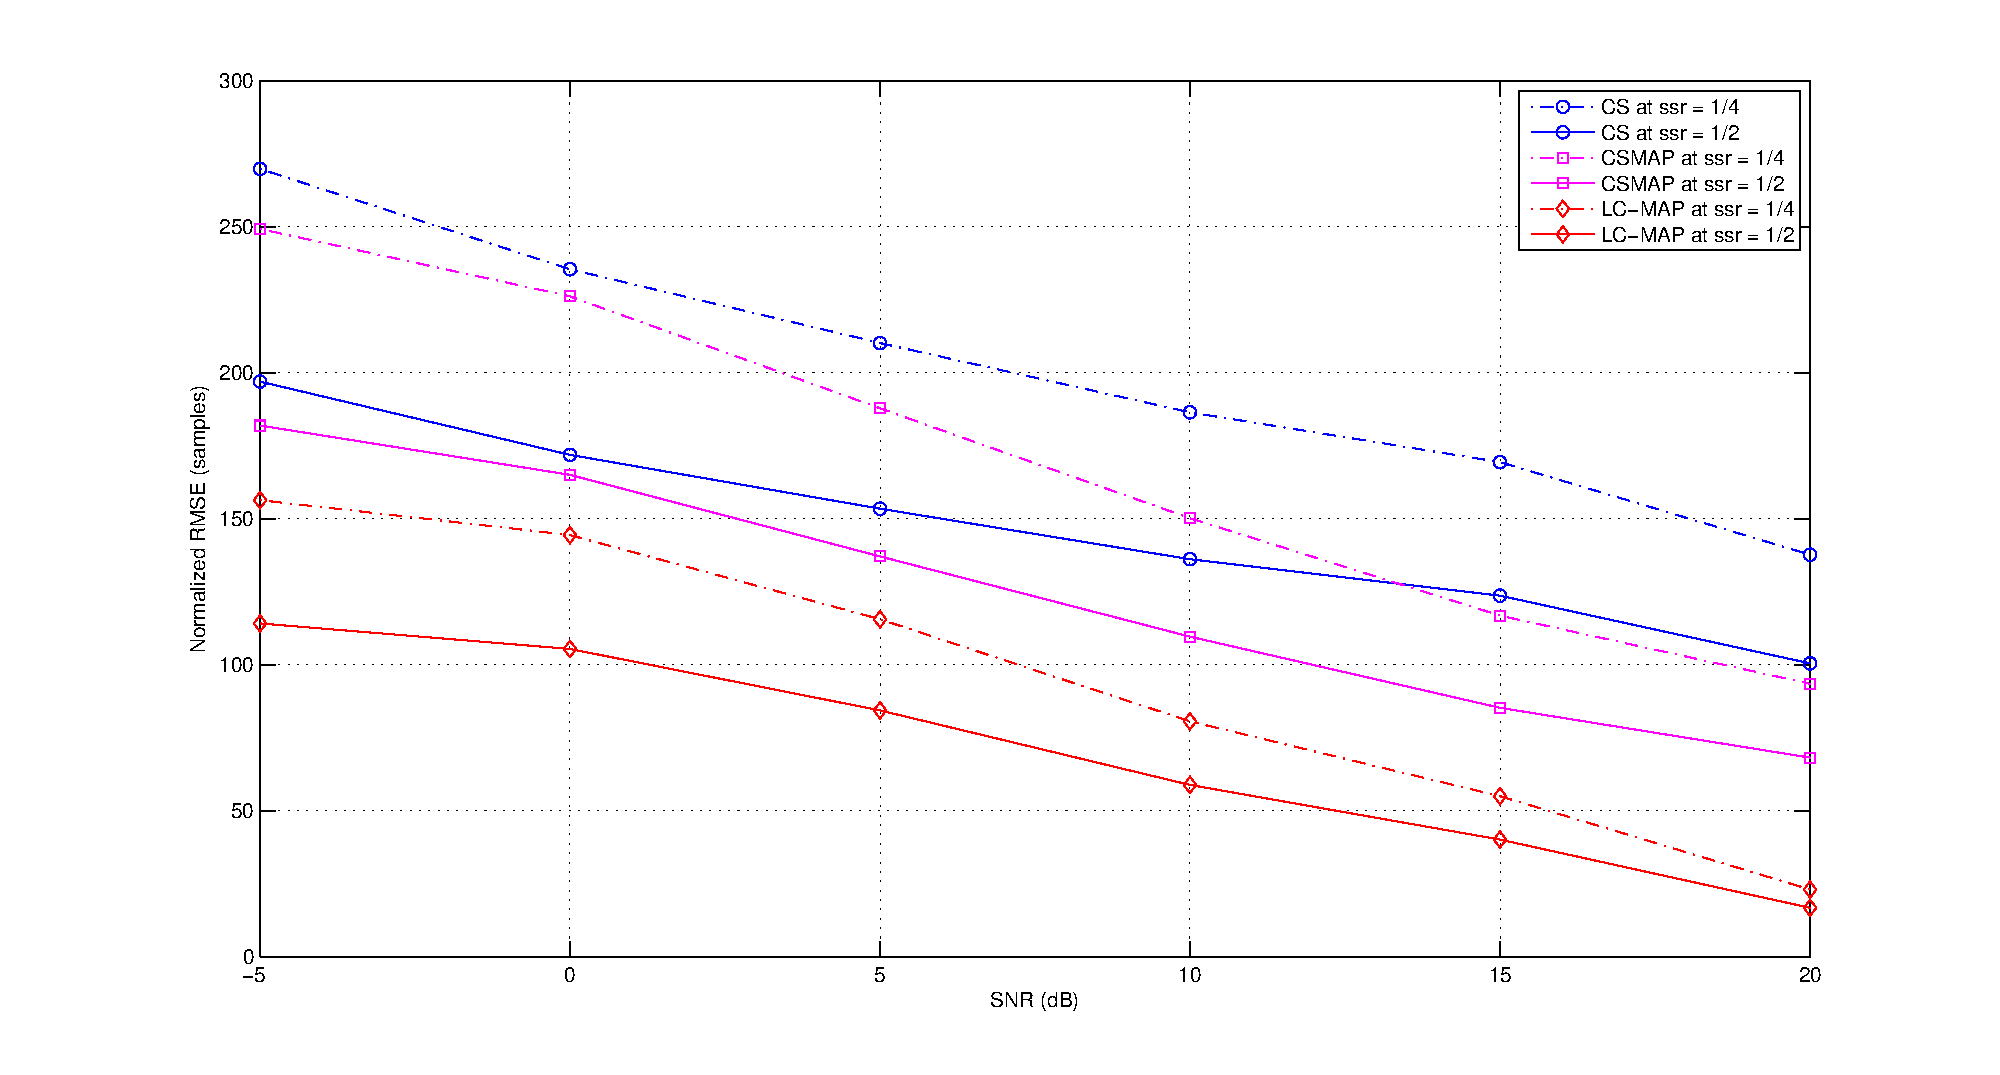
\includegraphics[width= 7.5cm, height= 5.26cm]{plot.pdf}
\caption{This is a plot to show the results.}
\label{fig:Plot}
\end{figure}
\newpage
{Enter material \cite{Zhang2004}.}
%
\begin{align}
\label{eq:TimeModel2a}
{r}(n \delta) &= {\sum_{l=0}^{L-1}a_l \mathit{g}(\delta - m_l \delta) + \omega(n \delta)}
\end{align}
%
The sub-sampled signal $\mathbf{y}$ at the receiver can be represented in the matrix form as
%
\begin{equation}
\label{eq:LinModel01}
\mathbf{y} = \mathbf{G} \mathbf{a} + \boldsymbol{\omega}
\end{equation}
%
{
where
%
\begin{equation}
\label{eq:P}
{\text{ \small $\mathbf{G}$}} = \left[
\begin{matrix}
\text{ \footnotesize $\mathit{g}(n-m_0)$}   & \ldots &   \text{ \footnotesize $\mathit{g}(n-m_N)$}\\
\text{ \footnotesize $\mathit{g}(n+{\mu}-m_1)$}   & \ldots &   \text{ \footnotesize $\mathit{g}(n+1-m_N)$}\\
%\vdots             & \ldots  & \vdots   \\
\vdots             & \ldots &  \vdots      \\
\text{ \footnotesize $\mathit{g}\left(n+{\mu}-m_M\right)$} & \ldots &   \text{ \footnotesize $\mathit{g}\left(n+\frac{M-1}{\mu}-m_N\right)$}
\end{matrix} \right]
\end{equation}
%

%%%%%%%%%%%%%%%%%%%%%%%%%%%%%%%%%%%%%%%%%%%%%%%%%%%%%%%%%%%%%%%%%%%%%%%%%%%%%%%%%%%%%%%%%%%%%%%%%%%%%%%%%%%

%% Please enter the Section Title in the following in place of xxxxx. Use a label in place of yyyyy to be
%% referred later.
%% Please write the text in between the braces in place of AAAAA

\section{Section Title}

{Enter material \cite{Tesi2006}.}

%%%%%%%%%%%%%%%%%%%%%%%%%%%%%%%%%%%%%%%%%%%%%%%%%%%%%%%%%%%%%%%%%%%%%%%%%%%%%%%%%%%%%%%%%%%%%%%%%%%%%%%%%%%

%% Please enter the Section Title in the following in place of xxxxx. Use a label in place of yyyyy to be
%% referred later.
%% Please write the text in between the braces in place of AAAAA

\section{Section Title}

{Enter material \cite{Gezici2009}.}

%% Sub-Sections are used if / where necessary.
%% Please enter the Sub-Section Title in the following in place of xxxxx. Use a label in place of yyyyy to
%% be referred later.
%% Please write the text in between the braces in place of AAAAA

\subsection{Sub-Section Title}

{Sub-section.}

%% Sub-Sub-Sections are used if / where necessary.
%% Please enter the Sub-Sub-Section Title in the following in place of xxxxx. Use a label in place of yyyyy
%% to be referred later.
%% Please write the text in between the braces in place of AAAAA

\subsection{Sub-Section Title}

{Sub-section \cite{Carbonelli2003}.}


%%%%%%%%%%%%%%%%%%%%%%%%%%%%%%%%%%%%%%%%%%%%%%%%%%%%%%%%%%%%%%%%%%%%%%%%%%%%%%%%%%%%%%%%%%%%%%%%%%%%%%%%%%%

%% Please enter the Section Title in the following in place of xxxxx. Use a label in place of yyyyy to be
%% referred later.
%% Please write the text in between the braces in place of AAAAA

\section{Section Title}

{Enter material \cite{Bajwa2010b}}

%%%%%%%%%%%%%%%%%%%%%%%%%%%%%%%%%%%%%%%%%%%%%%%%%%%%%%%%%%%%%%%%%%%%%%%%%%%%%%%%%%%%%%%%%%%%%%%%%%%%%%%%%%%

%% Please enter the Section Title in the following in place of xxxxx. Use a label in place of yyyyy to be
%% referred later.
%% Please write the text in between the braces in place of AAAAA

\section{Section Title}

{Enter section material.}
\newpage
\begin{table}[h]
\centering
\begin{tabular}{|c|c|c|c|c|c|c|}
\hline
Itr. No. & $\boldsymbol \Theta_n$ & Size of $\underline{\boldsymbol \alpha}_i$ & \multicolumn{4}{c|}{Residual: $r_i^n = \Vert \mathbf{y} \Vert_{\boldsymbol \Sigma_i}^{2}$ }\\ \cline{4-7}
$(n)$ & $(L \times n)$ & $(n \times 1)$ &
$i=1$ & $i=2$ & \dots \dots & $i=C$ \\
\hline
1 & $\boldsymbol \Theta_1 = [\boldsymbol \theta_1]$ & $(1 \times 1)$ & $r_1^1$
& $r_2^1$
& \dots \dots & $r_C^1$ \\
\hline
2 & $\boldsymbol \Theta_2 = [\boldsymbol \Theta_1 \boldsymbol \theta_2]$ & $(2 \times 1)$ &  $r_1^2$ & $r_2^2$
& \dots \dots & $r_C^2$  \\
\hline
3 & $\boldsymbol \Theta_3 = [\boldsymbol \Theta_2 {\boldsymbol \theta_3}]$ & $(3 \times 1)$ & $r_1^3$ & $r_2^3$
& \dots \dots & $r_C^3$  \\
\hline
\vdots & \vdots & \vdots & \vdots & \vdots & \dots \dots & \vdots \\
\vdots & \vdots & \vdots & \vdots & \vdots & \dots \dots & \vdots \\
\hline
$L-1$ & $\boldsymbol \Theta_{L-1} = [\boldsymbol \Theta_{L-2} {\boldsymbol \theta_{L-1}}]$ & $((L-1) \times 1)$ & $r_1^{L-1}$ & $r_2^{L-1}$
& \dots \dots & $r_C^{L-1}$\\
\hline
$L$ & $\boldsymbol \Theta_L = [\boldsymbol \Theta_{L-1} {\boldsymbol \theta_{L-1}}]$ & $(L \times 1)$ &  $r_1^L$ & $r_2^L$
& \dots \dots & $r_C^L$  \\
\hline
\end{tabular}
\caption{This is a Table.}
\label{tab:Table}
\end{table}

\end{document}

%%%%%%%%%%%%%%%%%%%%%%%%%%%%%%%%%%%%%%%%%%%%%%%%%%%%%%%%%%%%%%%%%%%%%%%%%%%%%%%%%%%%%%%%%%%%%%%%%%%%%%%%%%
%%%%%%%%%%%%%%%%%%%%%%%%%%%%%%%%%%%%%%%%%%%%%%%%%%%%%%%%%%%%%%%%%%%%%%%%%%%%%%%%%%%%%%%%%%%%%%%%%%%%%%%%%%
